\section{Fremdkapital}

\textbf{Unterschiede Eigenkapital vs. Fremdkapital}:
\begin{center}
	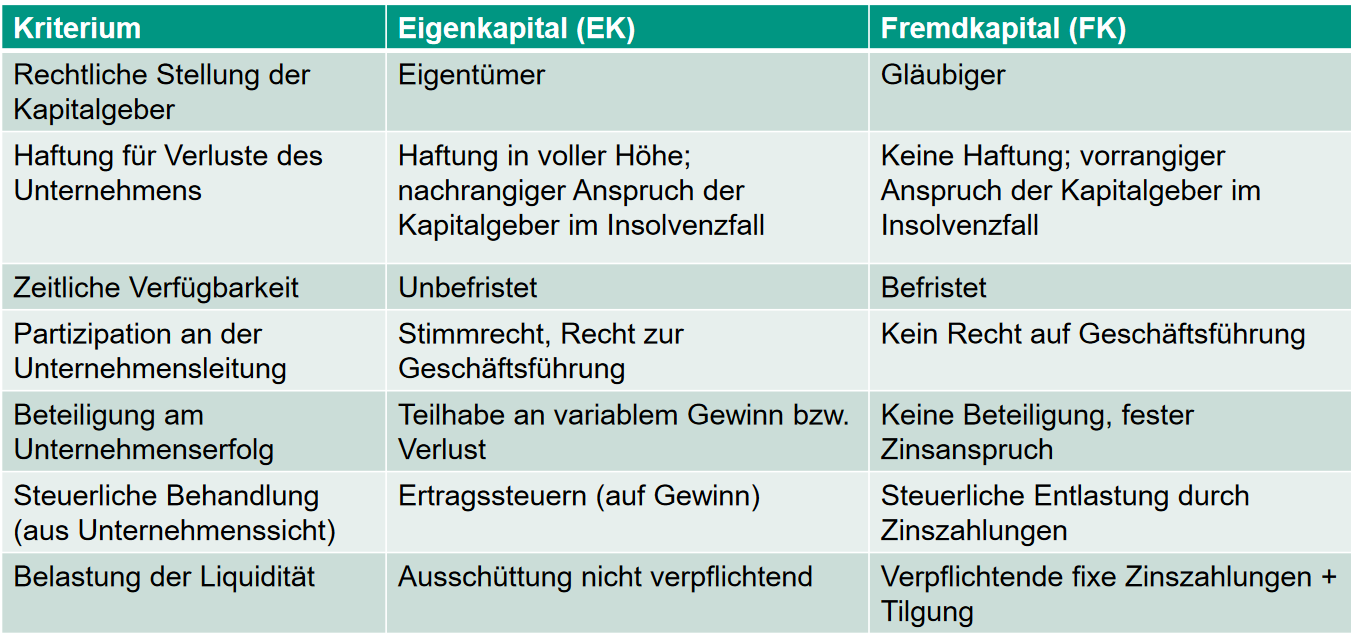
\includegraphics[width=0.8\textwidth]{images/ek-fk.png}
\end{center}

\textbf{Formen des Fremdkapitals}:
\begin{center}
	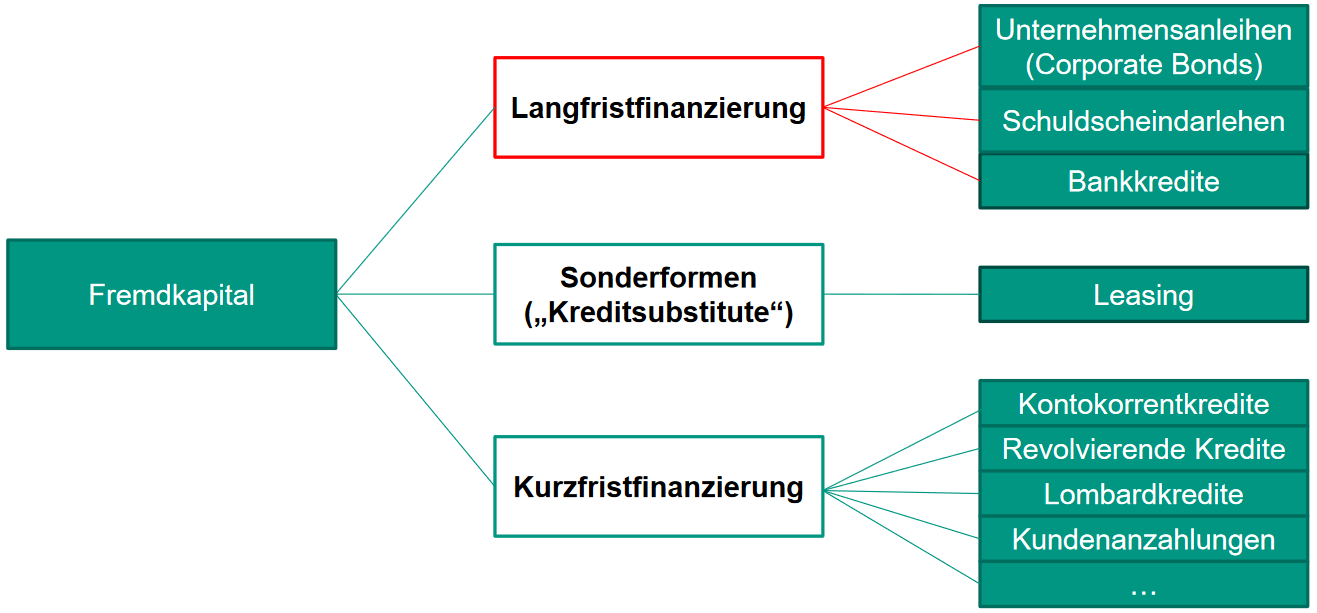
\includegraphics[width=0.6\textwidth]{images/formen-fk.png}
\end{center}

\textbf{Fremdkapitalkosten}: Fremdkapital können wegen den Zahlungsverpflichtungen Zahlungsreihen zugeordnet werden
\begin{center}
	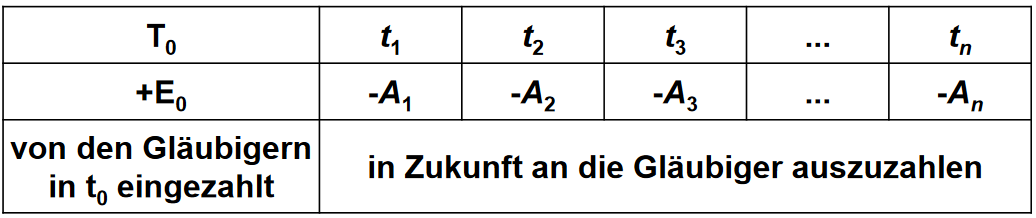
\includegraphics[width=0.5\textwidth]{images/fk-zr.png}
\end{center}
Einzahlungsbetrag $E_0$ von den Gläubigern bestimmt durch:
$$E_0=\sum\limits_{t=1}^{n}\frac{A_t}{(1+i)^t}\qquad\text{mit }i=\text{FK-Kostensatz, ermittelt als interner Zinssatz}$$
$\rightarrow$ Zusätzlich muss das Ausfallrisiko berücksichtigt werden\\

\textbf{Sicheres und unsicheres Fremdkapital}:
\begin{itemize}
	\item \textbf{Sicheres Fremdkapital}:
	\begin{itemize}
		\item $i$ ist der Kapitalmarktzinssatz für risikofreie Kapitalüberlassung
		\item $i$ orientiert sich am Zinssatz für risikolose Staatsanleihen
	\end{itemize}
\end{itemize}